\documentclass[handout]{beamer}
%\documentclass{beamer}

\usepackage{amsmath,graphicx,copyrightbox,pgfpages}
\pgfpagesuselayout{4 on 1}[letterpaper, landscape]

\usetheme{Dresden}
\usecolortheme{default}
\usefonttheme{serif}
\usefonttheme[onlylarge]{structuresmallcapsserif}
%\usefonttheme[onlysmall]{structurebold}

\title[Polytropes] % OPTIONAL: only for long titles
{Polytropic Models of White Dwarfs}
\subtitle{UNC PHYS 331 Project}
\author[Conn, Hurley] % OPTIONAL: for multiple authors
{Erin Conn \and Matthew Hurley}
\subject{Polytropes}
\date{April 14, 2014}

\AtBeginSection[]
{
        \begin{frame}<beamer>
            \frametitle{Table of Contents}
            \tableofcontents[currentsection]
        \end{frame}
}

\AtBeginSubsection[]
{
    \begin{frame}<beamer>
        \frametitle{Table of Contents}
        \tableofcontents[currentsection,currentsubsection]
    \end{frame}
}

% Small font sizes in image copyright notices
\makeatletter
\renewcommand{\CRB@setcopyrightfont}{%
    \usefont{T1}{phv}{m}{n}\fontsize{4}{4}\selectfont
}
\makeatother

\begin{document}

    \frame{\titlepage}

    \section{Theory}

        \subsection{Polytropes}

        \begin{frame}
            \frametitle{What are polytropes?}
            
            \pause
            Solutions to...

            \textbf{The Lane-Emden Equation}

            \[
                \frac{1}{\xi^2}\frac{d}{d\xi}\left(\xi^2\frac{d\theta}{d\xi}\right)=-\theta^n(\xi)
            \]

            A dimensionless, 2nd order nonlinear differential equation relating the
            pressure of a spherically-symmetric gas distribution to the radius.

        \end{frame}

        \begin{frame}
            \frametitle{Why polytropes?}

            \begin{itemize}
                \item Provide simplified stellar models - simple pressure/density relation
                    \pause
                \item Easier to solve than full equations of stellar structure
                    \pause
                \item Require less computational effort - some analytic solutions even exist!
            \end{itemize}

        \end{frame}

        \begin{frame}
            \frametitle{Definitions}

            \begin{definition}
                \alert{Polytropic fluid} - Fluid with an equation of state that depends on only one variable
                
            \end{definition} 
                    \pause
            \begin{definition}
                \alert{Polytropic index} - Constant that relates pressure of a polytropic fluid to its volume (density). It may be any real number.
            \end{definition}
            \pause
            \begin{definition}
                \alert{Poisson's equation} Relates a force density function to a potential field
                    \[\nabla^2\Phi=f\]
            \end{definition}

        \end{frame}

        \begin{frame}
            \frametitle{Derivation 1: Poisson Equation}
            % Skip this and the next 2 slides if pressed for time
            % Look up how to add skip buttons
            Can be derived multiple ways. From laws of mass conservation and
            hydrostatic equilibrium:
            \pause
            \[ \begin{array}{l l}
                dM(r) &= 4\pi r^2\rho(r)dr \rightarrow \frac{dM(r)}{dr}=4\pi r^2\rho(r) \\
                \pause
                \frac{dP(r)}{dr} &= -\frac{\rho(r)GM(r)}{r^2}
                \end{array}
            \]
            \pause
            These equations are related by multiplying the hydrostatic equation by
            \(r^2/\rho\) and differentiating:
            \pause
            \[\frac{d}{dr}\left(\frac{r^2}{\rho(r)}\frac{dP(r)}{dr}\right)=-G\frac{dM(r)}{dr}\]
            \pause
            Yielding Poisson's equation for gravity:
            \pause
            \[ \frac{1}{r^2} \frac{d}{dr} \left( \frac{r^2}{\rho(r)} \frac{dP(r)}{dr} \right) =-4 \pi G \rho(r) \]
        \end{frame}
        \begin{frame}
            \frametitle{Derivation 2: Working towards a dimensionless form}

            Define a polytropic state equation:
            \pause
            \[ P=K\rho^{\frac{n+1}{n}} \]
            \pause
            Make it dimensionless:
            \[\theta^n\equiv\frac{\rho}{\rho_c} \]
            \pause
            \[ P(r)=K\rho_c^{\frac{n+1}{n}}\theta^{n+1}(r)=P_c\theta^{n+1}(r) \]
            \pause
            Substitute into Poisson and simplify:
            \pause
            \[\frac{(n+1)P_c}{4\pi G\rho_c^2}\frac{1}{r^2}\frac{d}{dr}\left(r^2\frac{d\theta(r)}{dr}\right)=-\theta^n(r) \]

        \end{frame}

        \begin{frame}
            \frametitle{Derivation 3: More simplification}

            Define a new variable:
            \pause
            \[\alpha^2 \equiv \frac{(n+1)P_c}{4\pi G\rho_c^2}\]
            \pause
            Use it to define a dimensionless radius:
            \pause
            \[\xi \equiv \frac{r}{\alpha}\]
            \pause
            Substitute into the simplified Poisson:
            \pause
            \[\frac{1}{\xi^2}\frac{d}{d\xi}\left(\xi^2\frac{d\theta(\xi)}{d\xi}\right)=-\theta^n(\xi)\]

        \end{frame}

        \subsection{White Dwarfs}

        \begin{frame}
            \frametitle{Why White Dwarfs?}

            \begin{itemize}
                \item They are very dense
                \pause
                \item So dense that they are completely degenerate
                \pause
                \item We'll see why that's important shortly
            \end{itemize}

        \end{frame}

        \begin{frame}
            \frametitle{Definitions}

            \begin{definition}
                \alert{Degeneracy} - In quantum mechanics, when 2 or more energy
                states correspond to the same measured energy
            \end{definition}

            \begin{definition}
                \alert{Degenerate Matter} - Quantum version of an ideal gas.
                Appear under extremely high density or extremely low
                temperatures.
            \end{definition}

        \end{frame}

        \begin{frame}
            \frametitle{Degeneracy in White Dwarfs}

            \onslide<1-7>{High density results in complete degeneracy of
            electrons.}

            \only<2>{Pauli exclusion principle prevents more than 2 electrons in
            each}
            energy state.

            \onslide<3-5>{Density of electrons in with a range of momentum
            \([p,p+dp]\):

                \[ n_e(p,p+dp)\le \frac{8\pi p^2dp}{h^3}\] }

            \only<4>{ When \(n_e \ll \frac{8\pi p^2dp}{h^3}\), behaves as
            an ideal gas}

            \onslide<5-7>{As \(n_e \rightarrow \frac{8\pi p^2dp}{h^3}\),
            degeneracy increases and equation of state becomes:

                \[ P = K\rho^{\gamma}\]}

            \only<6>{As the density increases further, the electrons become
            relativistic.} 
            
            \only<7>{In the non-relativistic case, \(\gamma=5/3\). In the
            relativistic case, \(\gamma=4/3\).}

        \end{frame}

    \section{Methods}

        \begin{frame}
            \frametitle{Rearrange the Lane-Emden  Equation}

            \[\frac{d^2\theta}{d\xi^2}=-\frac{2}{\xi}\frac{d\theta}{d\xi}-\theta^n(\xi)\]

        \end{frame}

        \begin{frame}
            \frametitle{Translating to a system of 1st order equations}

            \[
                \left\{ \begin{array}{l l}
                \phi &= \frac{d\theta}{d\xi} \\
                \frac{d\phi}{d\xi} &= -\frac{2}{\xi}\phi - \theta^n
                \end{array} \right.
           \]

        \end{frame}

        \begin{frame}
            \frametitle{Boundary Values}

            Obtained from central density and hydrostatic equation

            % look up how to itemize & put in a box
            \[
                \begin{array}{l l}
                    \xi &= 0 \\
                    \theta &= 1 \\
                    \frac{d\theta}{d\xi} &= 0
                \end{array}
            \]

        \end{frame}

        \begin{frame}
            \frametitle{Runge-Kutta Solution}

            Used a 4th degree Runge-Kutta solver

            Did not know the integration range beforehand:

            To find the surface with arbitrary precision, backed up a step and
            halved the step size if \(\theta<0\) until desired precision reached

        \end{frame}

        \begin{frame}
           \frametitle{Problem!}

            Singularity at \(\xi_0=0\):

            \[ \phi'=-\left(\frac{2}{\xi_0}\phi\right)-\theta_0^n\]

            Need to work around this somehow:
            \pause
            \begin{itemize}
                \item Taylor expand at \(\xi=0\) and take limit as \(\xi\rightarrow 0\): \(\phi'\rightarrow -\frac{1}{3}\)
                \pause
                \item Offset the starting point: \(0< \xi_0 \ll 1\)
            \end{itemize}

        \end{frame}

        \begin{frame}
            \frametitle{Getting something useful}

           Finding the density \& pressure:

           \[\frac{\rho}{\rho_c} = \frac{1}{3}\frac{\xi_f}{\theta(\xi_f)}\]

        \end{frame}

    \section{Results}

        \begin{frame}
            \frametitle{Solutions for n=1.5 and n=3}

            \only<1>{
                Parameters for n=1.5, 3 polytropes\cite{hansen2004}
                \begin{tabular}{c | c c c}
                    $n$ & $\xi_f$ & $\theta'(\xi_f)$ & $\rho_c/\langle\rho \rangle$ \\
                    \hline
                    1.5 & 3.6538 & -0.20330 & 5.991 \\
                    3 & 6.8969 & -0.04243 & 54.1825
                \end{tabular}
            
                \pause

                Our calculated values:
                \begin{tabular}{c | c c c}
                    $n$ & $\xi_f$ & $\theta'(\xi_f)$ & $\rho_c/\langle\rho \rangle$ \\
                    \hline
                    1.5 & 3.6538 & -0.2033 & 5.9907 \\
                    3 & 6.8968 & -0.0424 & 54.1825
                \end{tabular}
            }
            \only<2>{
            \copyrightbox[b]
                {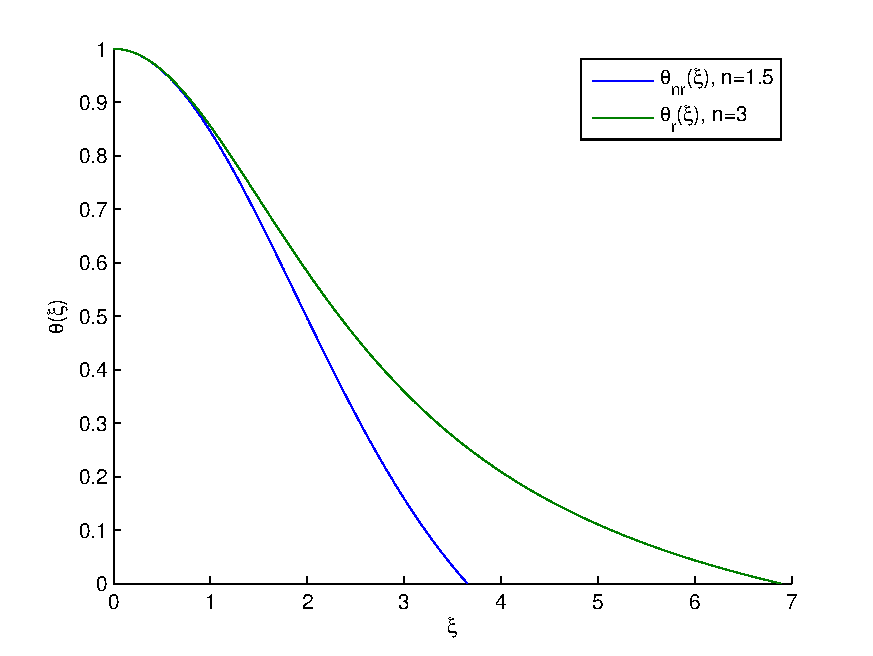
\includegraphics[width=0.8\textwidth]{lesolution.pdf}}
                {Image created by presenters in Matlab}
            }

        \end{frame}

        \begin{frame}
            \frametitle{Density Profile}

            \copyrightbox[b]
                {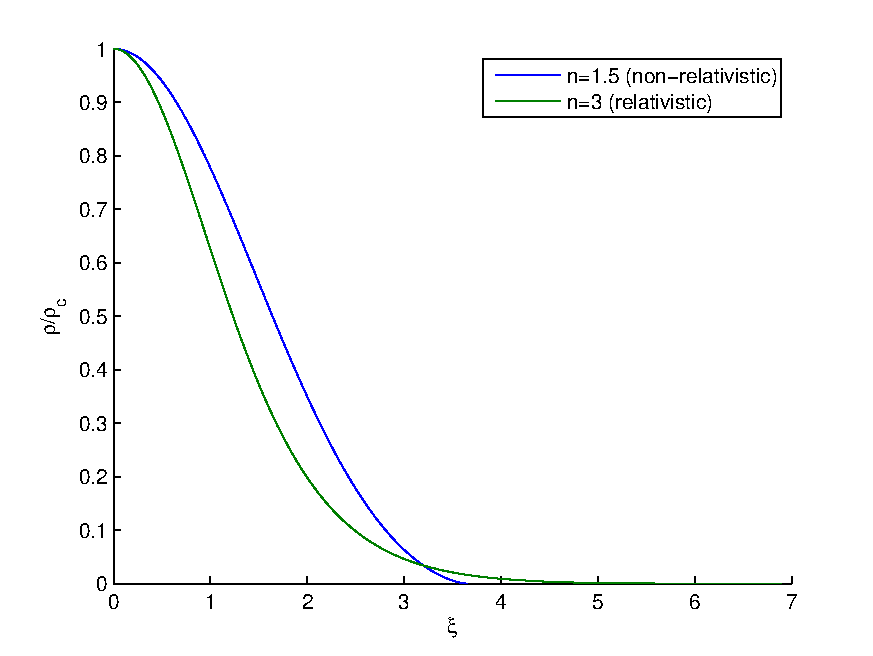
\includegraphics[width=0.8\textwidth]{density.pdf}}
                {Image created by presenters in Matlab}

        \end{frame}

        \begin{frame}
            \frametitle{Mass - Radius Relationship}

            \only<1>{ We did not get this working correctly yet. We believe
            we're having trouble with unit conversions}

            \only<2>{
                \copyrightbox[b]
                    {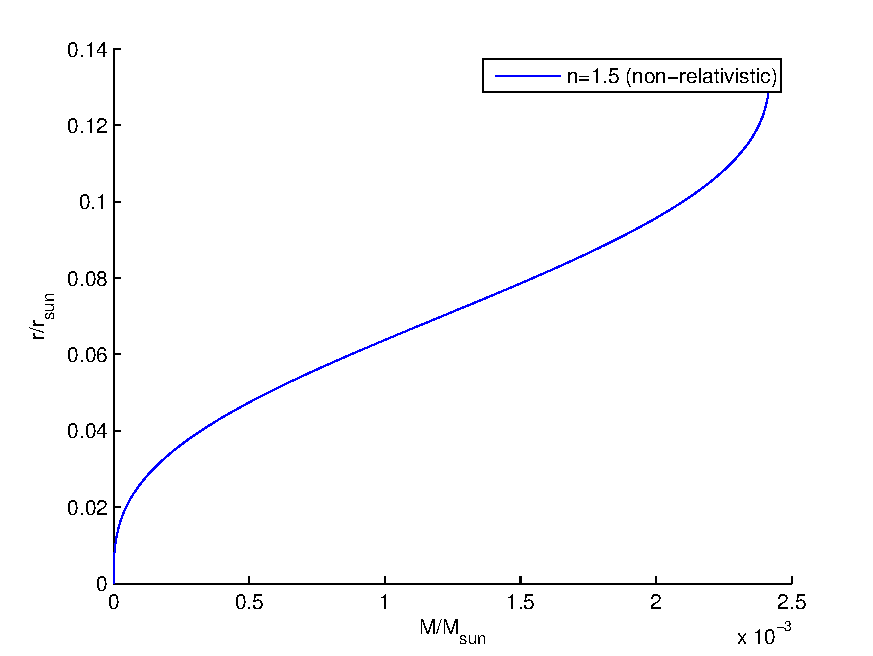
\includegraphics[width=0.8\textwidth]{mr-nonrel.pdf}}
                    {Image created by presenters in Matlab}
            }
            \only<3>{
                \copyrightbox[b]
                    {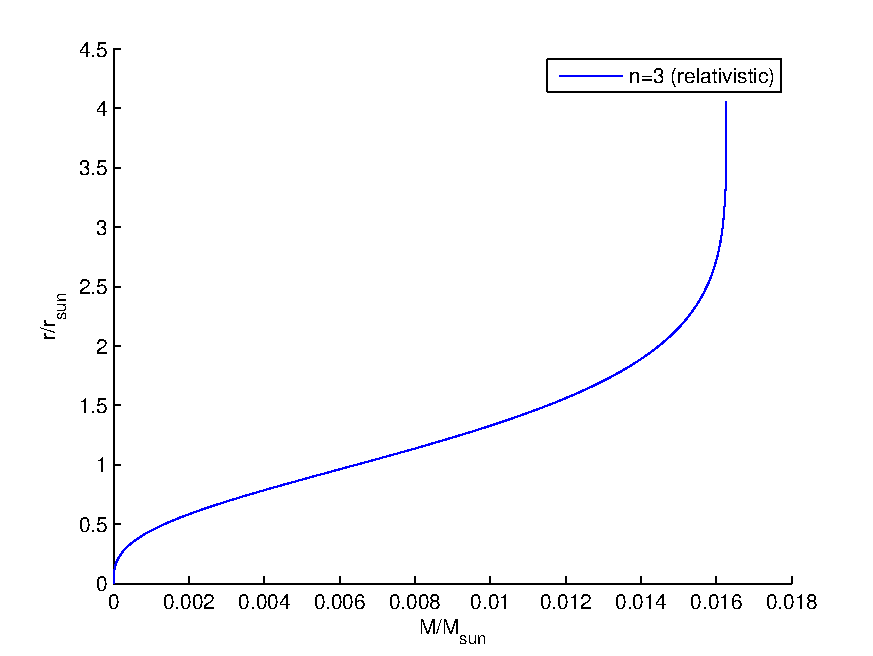
\includegraphics[width=0.8\textwidth]{mr-rel.pdf}}
                    {Image created by presenters in Matlab}
            }
            \only<4>{
                \copyrightbox[b]
                    {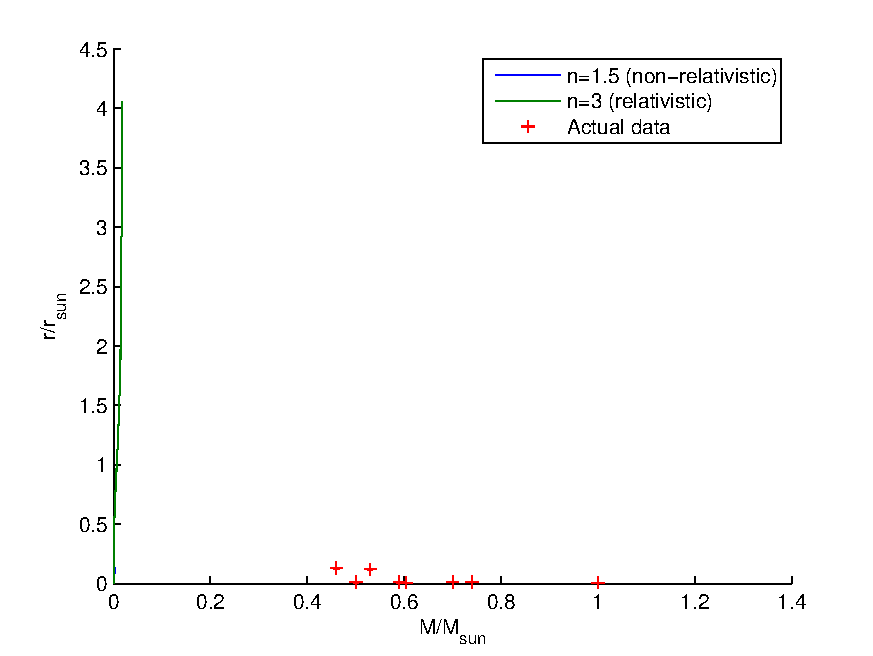
\includegraphics[width=0.8\textwidth]{mr-data.pdf}}
                    {Image create by presenters in Matlab, Data from astronomical surveys of white dwarfs in binary systems}
            }

        \end{frame}

    \section{Discussion}

        \begin{frame}
            \frametitle{Challenges}

                \only<1>{
                \begin{itemize}
                    \item Major difficulty was in correctly framing the problem. 
                    \item Initially tried to use a shooting method - but with
                    free boundary it became prohibitively difficult.
                    \item Rearranged \& used known physics to turn into initial
                    value problem.
                \end{itemize}
                }

                \only<2>{
                    \begin{itemize}
                        \item Computing the mass-radius relationship
                        \item Sources differed on derivation
                        \item UNITS
                     \end{itemize}
                }

        \end{frame}

        \begin{frame}
            \frametitle{Where to go from here?}

            Fix our calculation of the mass-radius relationship

            Real white dwarfs have a mixed equation of state; non-relativistic
            near surface and highly relativistic near core. 

            Approximate this state equation to find behavior near Chandrasekhar
            mass

        \end{frame}

        \begin{frame}
            \frametitle{Questions?}

            \copyrightbox[b]
                {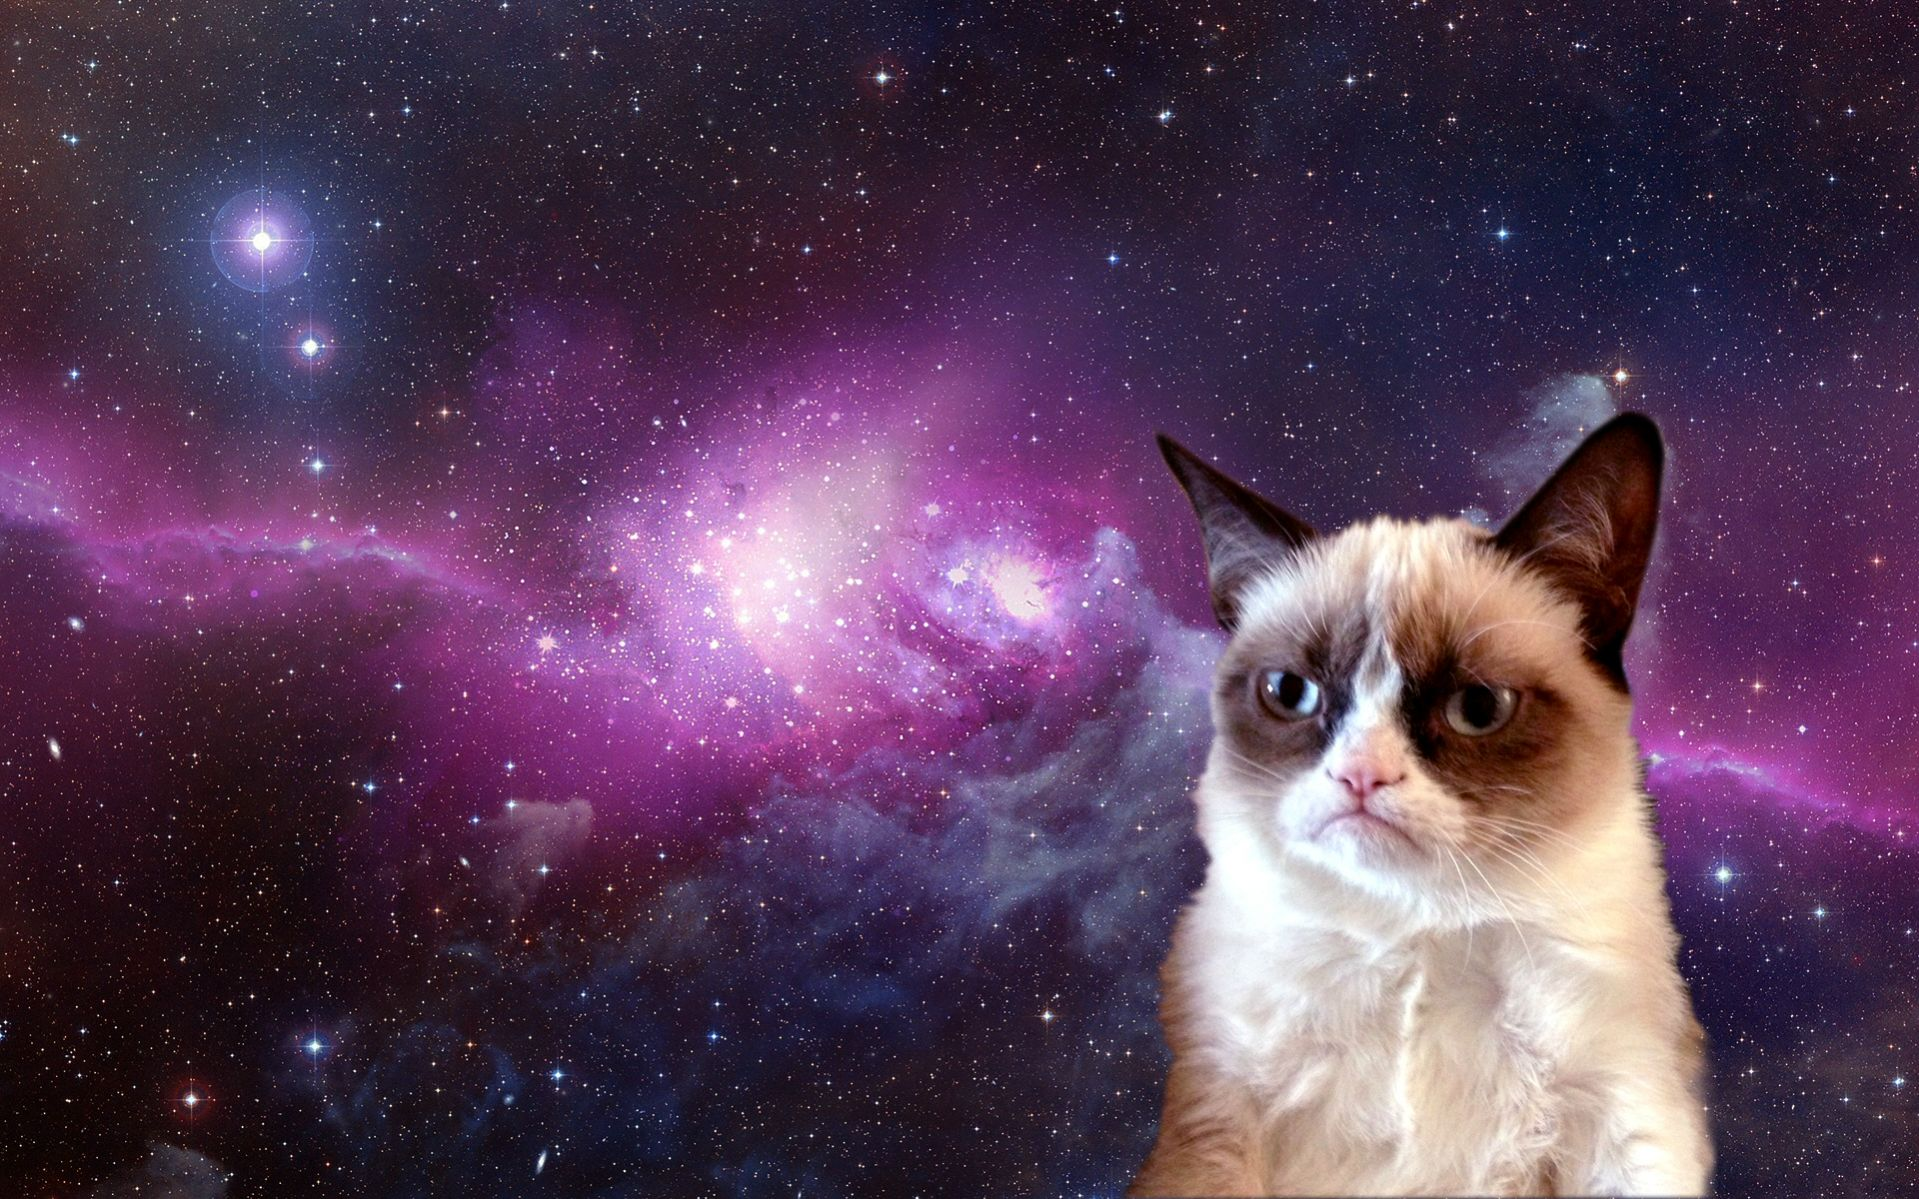
\includegraphics[width=\textwidth]{Grumpy-Cat-in-Space.jpg}}
                {Copyright by Abe, http://downloadwallpaperhd.com Non-commercial use only}

        \end{frame}

    \section{References}

        \begin{frame}[allowframebreaks]
            \frametitle{References}
            \begin{thebibliography}{10}

                \beamertemplatebookbibitems

                \bibitem{hansen2004}
                    C. Hansen, S. D. Kawaler, V. Trimble.
                    \newblock {\em Stellar interiors: physical principles, structure, and evolution}.
                    \newblock Springer-Verlag, 2004.

                \bibitem{leblanc2010}
                    F. LeBlanc
                    \newblock {\em An introduction to stellar astrophysics}.
                    \newblock John Wiley \& Sons, 2010.

                \bibitem{jardetsky1958}
                    W. S. Jardetsky.
                    \newblock {\em Theories of figures of celestial bodies}.
                    \newblock Dover Publications, 1958.

                \beamertemplatearticlebibitems

                \bibitem{website:wolfram}
                    E. W. Weisstein.
                    \newblock {\em Lane-Emden differential equation}.
                    \newblock \url{http://mathworld.wolfram.com/Lane-EmdenDifferentialEquation.html}

                \bibitem{website:dhillon}
                    V. Dhillon.
                    \newblock Solving the Lane-Emden equation
                    \newblock {\em PHY 213 - The structure of main-sequence stars}
                    \newblock \url{http://www.vikdhillon.staff.shef.ac.uk/teaching/phy213/phy213\_le.html}


            \end{thebibliography}

        \end{frame}

\end{document}
